\section*{Problem 7}

Use the FFT to approximate the Fourier Transform of $x(t) = 4e^{-t}u(t)$. 
Consider the following cases:

\begin{enumerate}
\item Sampling period T = 1, N = 10.
\item Sampling period T = 1, N = 20.
\item Sampling period T = 0.5, N = 20.
\item Sampling period T = 0.1, N = 100
\end{enumerate} 

\subsection*{Solution}

The fourier transform of $x(t)$ is:

\begin{equation*}
\begin{aligned}
X(\omega) = \frac{1}{1 +j \omega}
\end{aligned}
\end{equation*}

In order to approximate $X(\omega)$ using the $FFT$, the following
equation must be used \cite{kamen2000fundamentals}:

\begin{equation}
X(k\Gamma) = \frac{1 - e^{-j k \Gamma T}}{j k \Gamma} X_k
\label{eq:fftapprox}
\end{equation} 

Where $\Gamma = \frac{2\pi k}{N T}$ and $X_k$ is the output from the $FFT$ with $k=0,1,..,N-1$.

\zcodemat{sources/c4p7.m}{Mlab for plotting $X(\omega)$ and its approximation using $FFT$}

\begin{figure}[H]
\caption{Plot of $X(\omega)$ and approximation using $FFT$ for different $T$}
\centering
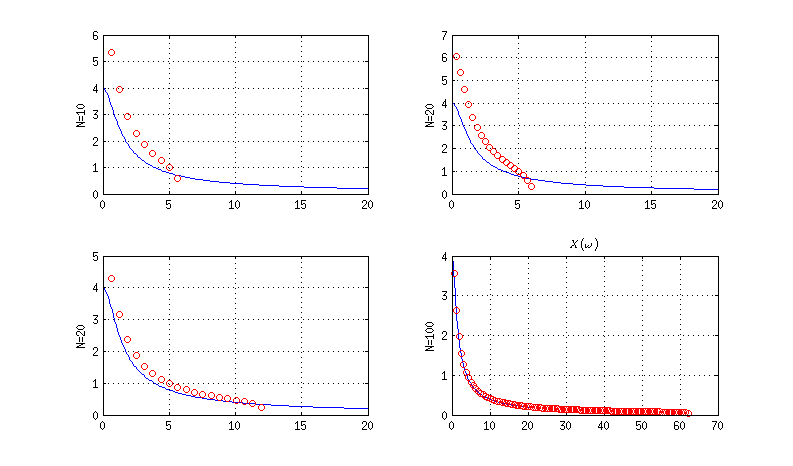
\includegraphics[width=0.8\textwidth]{figs/c4p7.png}
\label{fig:c4p7}
\end{figure}

